\chapter{Le routage}\label{ch:routage}
 
  \section{Présentation}
Le routage est le mécanisme qui gère les tables de routage et choisit l’itinéraire à suivre dans le réseau afin d’acheminer des paquets. Le routage peut se faire vers un ou plusieurs destinataires (multicast : \ref{sc:rout_multicast}) en utilisant un algorithme de routage approprié.

  \subsection{Algorithme de routage}
L’algorithme de routage décide du routage à suivre pour les paquets entrants et gère les tables de routage. 
\medskip

L’algorithme de routage doit être apte à s’adapter à toutes variations du réseau (défaillance matérielle et logicielle, modification rapide de la topologie du réseau, congestion). Il doit se montrer efficace au niveau local et global (maximiser l’efficacité globale peut être opposé à maximiser l’efficacité locale) et doit donc faire des compromis.
\\
Un algorithme de routage peut être statique ou dynamique. 
Dans le cas dynamique, l’algorithme construit la table de routage automatiquement en échangeant des informations au sein du réseau alors que dans le cas statique, la table doit être implémentée et modifiée manuellement.
\medskip

Nous nous intéresserons aux algorithmes de routage dynamiques, en particulier, le routage par vecteur de distance et le routage par informations d’état de lien. 

  \subsubsection{Routage par vecteur de distance (Distance vector)}\label{sc:rout_vect}
Le routage par vecteur de distance fonctionne par le principe de collaboration entre routeurs directement voisins. Chaque routeur a une table de routage contenant l’adresse de l’émetteur et du destinataire et le coût associé (dépend de plusieurs paramètres : nombre de saut, degré de congestion, temps de transit estimé). Les routeurs vont communiquer périodiquement (hello-time) le contenu de leur table de routage (update).

\begin{figure}[h]
    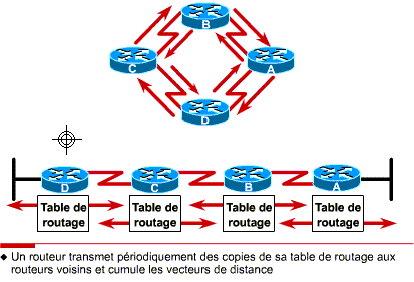
\includegraphics[width=270px]{figures/routage_vect.png}
    \centering
    \caption{Routage par vecteur de distance \cite{Rout_vecteur}}
    \end{figure}

Le routeur va ainsi pouvoir actualiser sa table de routage et prendre en compte les modifications du réseau (nouvelles destinations, coût modifié, panne).
\medskip

Suivant la destination qu’un paquet doit prendre, le routeur va consulter sa table de routage et emprunter la destination au coût le plus faible. Ainsi, la distance pour arriver à destination est calculée pas à pas et le routeur n’a pas connaissance de la topologie entière du réseau.
\medskip

Les désavantages des protocoles à vecteurs de distance sont :

	\begin{itemize}
	\item La charge réseau par les updates
    \item Le délai de convergence 15: un délai non négligeable est nécessaire pour savoir qu’un voisin est définitivement déconnecté (panne ou non). 
    \\
    Cet algorithme n’est donc pas efficace pour gérer un réseau à la topologie non stable.
    \item La latence : un certain délai est nécessaire pour actualiser la table de routage si le réseau est grand.
	\end{itemize}

  \subsubsection{Routage par informations d’état de lien (Link State)}\label{sc:rout_lien}
Contrairement à l’algorithme précédent, le routage par informations d’état de lien va chercher à comprendre la topologie complète du réseau, ce qui répond aux limitations du routage vecteur de distance.
\\
Cet algorithme se déroule en cinq points :
\begin{itemize}
\item Découverte des voisins du routeur : communique avec les voisins directs afin d’obtenir leur adresse et prise en compte des LAN à diffusion (réseau diffusant une information à tous les routeurs connectés du LAN) où il est seulement nécessaire de connaître une adresse du LAN.
\item Définition des coûts de lien : associe une adresse à un coût qui dépend de la distance, du débit et temps de transit estimé afin de trouver le chemin le plus optimal (au coût moindre).
\item Élaboration des paquets d’états de lien : Dès que le routeur possède les informations nécessaires sur ses voisins, il transmet un paquet d’états de lien à tous ses voisins qui renseigne l’état du réseau à proximité direct du routeur.
\\
Le paquet contient l’adresse de l’émetteur, un numéro de séquence, un âge, et l’adresse de ses voisins associés à leur coût. Il faut aussi décider de la fréquence d’envoi de ces paquets (par période fixe ou lors d’une modification du réseau).
\item Distribution des paquets d’états de lien : Assure l’envoi et la réception des paquets d’états de lien à tous les routeurs, et rapidement. Cette étape gère les numéros de séquence ainsi que l’âge des paquets afin d’éviter toute duplication.
\item Calcul de nouvelles routes : Dès que le routeur a reçu tous les paquets d’états de lien, il va pouvoir représenter le réseau dans son ensemble par un graphe. Ensuite, il suffit d’appliquer l’algorithme de Dijkstra sur le graphe qui va calculer le plus court chemin.
\end{itemize}
\medskip

Le principal désavantage de cet algorithme est qu’il est gourmand en capacité mémoire (chaque routeur a connaissance du réseau en entier) et calcul (il faut régulièrement calculer le plus court chemin du graphe).
Cependant, il est réactif aux variations du réseau.


  \section{Les protocoles de routage}
Nous allons traiter deux protocoles de routage intradomaine (protocole de passerelle intérieure) très répandus. 

  \subsection{Le protocole RIP (RIPng : Routing Information Protocol)}\label{sc:ripng}
Le protocole de routage RIP se base sur le routage par vecteur de distance (\ref{sc:rout_vect}). De ce fait, il possède les mêmes défauts et fonctionne sous le même principe, mais introduit une limite de coût : 15, afin d’éviter les boucles de routage. RIPng inclut les masques sous-réseau dans les updates pour les réseaux qui en ont besoin (VLMS : Variable Length Masque Subnet).
\\
Il supporte l’IPv6.
\\
L’adresse multicast utilisée est \textit{224.0.0.9}.

    \begin{figure}[h]
    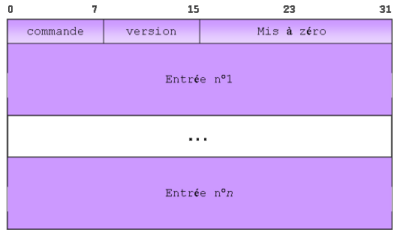
\includegraphics[width=270px]{figures/RIPvng_paquet.png}
    \centering
    \caption{Format d'un paquet RIPng \cite{Xripng}}
    \end{figure}

    \begin{figure}[H]
    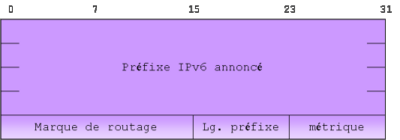
\includegraphics[width=270px]{figures/RIPvng_entree.png}
    \centering
    \caption{Champ entrée d'un paquet RIPng \cite{Xripng}}
    \end{figure}

Il n’est pas adapté aux grands réseaux.

  \subsection{Le protocole OSPF (OSPFv3 : Open Shortest Path First)}
Le protocole de routage OSPF se base sur le routage par état de lien (\ref{sc:rout_lien}). Il répond aux défauts du protocole RIP.
\\
Voici les services apportés par le protocole :
    \begin{itemize}

    \item Protocole ouvert donc non propriétaire.
    \item Routage par type de service : il est possible de spécifier un type de service dans les paquets.
    \item Permet la division du réseau en aires autonomes et indépendantes entre elles. L’interface entre deux aires est nommée l’aire backbone, ce qui permet d’optimiser le routage en communiquant des résumés de route ainsi que la nature des réseaux IP. Chaque routeur a donc connaissance de la topologie de son aire.
    \item Gère le routage machine-machine, vers réseaux et sous-réseaux.
    \item Utilise l’adressage multicast IP (voir \ref{sc:@multicast}).
    \item Réactif aux variations du réseau (panne, congestion…) et optimal : car basé sur le routage par état de lien. Il tient compte du trafic afin de ne pas envoyer tous les paquets sur la meilleure route et de ne pas délaisser les autres routes possibles.
    \item Peut évaluer une variété de types de coût (nombre de sauts, débit…). 
    \item Supporte VLMS (comme RIPng (\ref{sc:ripng})).
    \item Supporte l’IPv6 (voir \ref{ch:ipv6}).

    \end{itemize}
\medskip

OSPF utilise cinq types de messages différents :

\begin{figure}[H]
    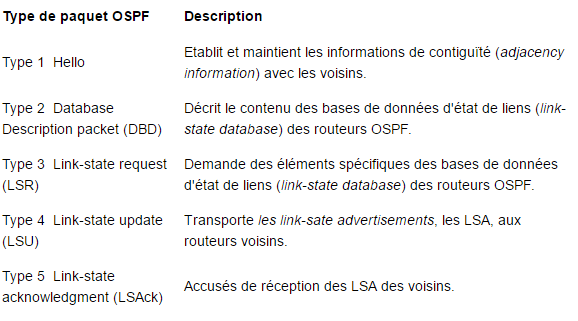
\includegraphics[width=340px]{figures/OSPF_type_paquet.PNG}
    \centering
    \caption{Type de paquet OSPF \cite{Xospf}}
    \end{figure}
    
Ce protocole est rapide, robuste aux variations du réseau, interopérable et permet de gérer des paramètres utiles à la QoS (\ref{ch:qos}) (répartition du trafic, prise en compte du type de service…).
\\
Il possède les mêmes défauts que le routage par état de lien (\ref{sc:rout_lien}), mais la répartition par aire complique la configuration.

  \section{Le routage multicast}\label{sc:rout_multicast}
  
  \subsection{Les besoins}
Une application requiert de diffuser des données en continu à un groupe particulier de personnes, comme le streaming vidéo en direct d’un concert et plus généralement, la téléconférence. Dans cet exemple, un émetteur unique transmet un flux d’information à un public visé. Pour ce faire, il faut utiliser le routage multicast.

  \subsection{Les difficultés}
Toute la difficulté du routage multicast réside dans la diffusion efficace de l’information au groupe concerné.
\\
Cela requiert donc un routage performant.
\\
L’efficacité de la diffusion dépend de deux cas de figure :
  \begin{itemize}
  \item Le groupe est dense : les membres du groupe sont dispersés sur une majeure partie du réseau.
  \item Le groupe n’est pas dense : beaucoup d’éléments du réseau ne font pas partie du groupe.
  \end{itemize}

  \subsection{Quelles solutions ?}
Pour communiquer à plusieurs membres particuliers du réseau, plusieurs techniques existent. Elles consistent toutes à obtenir le graphe du groupe de diffusion sans boucles (arbre du groupe) par élagage du graphe du réseau sans boucles (arbre recouvrant).

  \subsubsection{Avec un routage par état de lien}
Dans ce cas, la topologie complète du réseau est connue par chaque routeur. Il est ainsi facile de construire un graphe contenant le réseau sans les éléments qui ne sont pas membres du groupe ainsi que leurs liens.
\\
Cela permet d’obtenir un graphe spécifique au groupe de diffusion.

  \subsubsection{Avec un routage par vecteur de distance (DVMRP : Distance Vector Multicast Routing Protocol)}
  Cette solution se base sur le protocole RIP (\ref{sc:ripng}).
  \\
En trois étapes :
    \begin{itemize}
    \item Un premier message pour le groupe est envoyé sur le réseau. Le champ TTL (time to live) du message restreint la zone de diffusion de ce dernier.
    \item Tous les routeurs recevant ce message, mais ne faisant pas partie du groupe multicast et n’étant pas liés directement à un membre renvoient un message PRUNE à l’émetteur. Ce message précise qu'un routeur n’est pas membre du groupe et ne veut plus recevoir de message de ce groupe.
    \item À partir de la réponse de chacun des récepteurs, il est ainsi possible de construire un arbre du groupe multicast.
    \end{itemize}
\medskip

L’arbre obtenu ne contient que les liaisons utiles pour diffuser un message sur le groupe multicast. Il est donc efficace.
\\
Cependant, le problème est que cela nécessite une grande capacité de travail pour chaque routeur, en particulier dans les grands réseaux. En effet, il faut constituer et mémoriser un arbre pour chaque routeur membre du groupe dans un réseau de taille supérieur ou égal.

  \subsubsection{Avec la technique du coeur de l'arbre (CBT : Core-based tree)}
Dans ce cas, un seul arbre est calculé par groupe et chaque routeur membre en a connaissance.
\\
Le principe est de décider d’un routeur racine (membre du groupe) : le cœur. L’arbre obtenu par cette technique est le CBT.
\medskip

Le cœur doit d’abord constituer le CBT. Chaque membre envoie un paquet vers le cœur, ce qui permet d’obtenir la route entre le cœur et chaque membre du groupe. L’arbre du groupe a donc le cœur comme racine et tous ses membres en branches et feuilles.

\begin{figure}[h]
    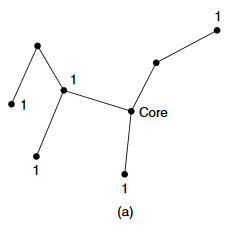
\includegraphics[width=160px]{figures/cbt.PNG}
    \centering
    \caption{Core-based tree}
    \end{figure}

Le choix de la racine est critique pour la performance.
\\
Cette technique est très optimale si le cœur est au milieu de l’arbre, et donc à distance plus ou moins égale de chaque membre du groupe. Elle se montre utile dans le cas où le groupe est dispersé dans le réseau.
\\
De plus, seul un arbre est nécessaire pour chaque membre du groupe et ceux qui ne sont pas membres du groupe ne travaillent pas. Ainsi, on gagne en capacité mémoire et calcul.